% answers.tex —— 2005 年·全国卷Ⅰ·文科 · 参考答案与详细解析片段
% 由 tools/generate_projects.py 依来源总账自 2005/2005_数学真题_全国1文_试题.md + 2005/2005_数学真题_全国1文_解析正文.md + 2005/2005_数学真题_全国1文_答案要点.md 生成，勿手改（改源 MD 后重跑）


\begin{gktip}
固定源 PDF 为印刷页码 248–249 的两页题面，不附答案。以下解析均依据固定源独立复算；第 4、18 题图形在 LaTeX 工程中以 TikZ/PGFPlots 矢量源重绘。
\end{gktip}

\begin{answer}
\gksolhead{1}{}

\textbf{题目}：

设 $I$ 为全集，$S_1\text{、}S_2\text{、}S_3$ 是 $I$ 的三个非空子集且 $S_1\cup S_2\cup S_3=I$，则下面论断正确的是\mbox{（　　）}

（A）$\complement_I S_1\cap(S_2\cup S_3)=\varnothing$\quad（B）$S_1\subseteq(\complement_I S_2\cap\complement_I S_3)$

（C）$\complement_I S_1\cap\complement_I S_2\cap\complement_I S_3=\varnothing$\quad（D）$S_1\subseteq(\complement_I S_2\cup\complement_I S_3)$

\Needspace{4\baselineskip}
\textbf{解析}

\Needspace{5\baselineskip}
由 $S_1\cup S_2\cup S_3=I$，不存在同时不属于三个集合的元素，因此

\nopagebreak[4]
\[
\complement_I S_1\cap\complement_I S_2\cap\complement_I S_3=\varnothing\text{。}
\]

\gkanswer{答案：C}

\end{answer}
\begin{answer}
\gksolhead{2}{}

\textbf{题目}：

一个与球心距离为 $1$ 的平面截球所得的圆面面积为 $\pi$，则球的表面积为\mbox{（　　）}

（A）$8\sqrt2\pi$\quad（B）$8\pi$\quad（C）$4\sqrt2\pi$\quad（D）$4\pi$

\Needspace{4\baselineskip}
\textbf{解析}

\Needspace{5\baselineskip}
截面圆半径为 $1$，球心到截面平面的距离为 $1$，所以球半径满足

\nopagebreak[4]
\[
R^2=1^2+1^2=2\text{。}
\]

球的表面积为 $4\pi R^2=8\pi$。

\gkanswer{答案：B}

\end{answer}
\begin{answer}
\gksolhead{3}{}

\textbf{题目}：

函数 $f(x)=x^3+ax^2+3x-9$，已知 $f(x)$ 在 $x=-3$ 时取得极值，则 $a=$\mbox{（　　）}

（A）$2$\quad（B）$3$\quad（C）$4$\quad（D）$5$

\Needspace{4\baselineskip}
\textbf{解析}

\nopagebreak[4]
\[
f'(x)=3x^2+2ax+3\text{。}
\]

\Needspace{5\baselineskip}
极值点 $x=-3$ 必须满足 $f'(-3)=0$，即

\nopagebreak[4]
\[
27-6a+3=0,
\]

故 $a=5$。

\gkanswer{答案：D}

\end{answer}
\begin{answer}
\gksolhead{4}{}

\textbf{题目}：

如图，在多面体 $ABCDEF$ 中，已知 $ABCD$ 是边长为 $1$ 的正方形，且 $\triangle ADE\text{、}\triangle BCF$ 均为正三角形，$EF\parallel AB$，$EF=2$，则该多面体的体积为\mbox{（　　）}
\nopagebreak[4]
\begin{center}% 2005 年全国卷Ⅰ文科第 4 题：多面体 ABCDEF
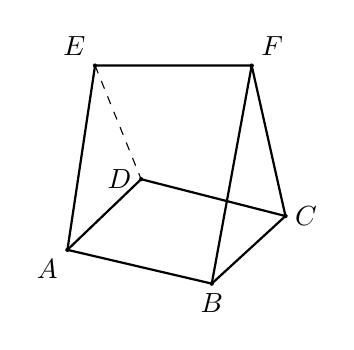
\begin{tikzpicture}[>=stealth,scale=0.78]
  \coordinate (A) at (0,0); \coordinate (B) at (2.35,-0.55);
  \coordinate (C) at (3.55,0.55); \coordinate (D) at (1.2,1.15);
  \coordinate (E) at (0.45,3.0); \coordinate (F) at (3.0,3.0);
  \draw[thick] (A)--(B)--(C)--(D)--cycle;
  \draw[thick] (A)--(E)--(F)--(B);
  \draw[thick] (C)--(F);
  \draw[dashed] (E)--(D) (D)--(C);
  \fill (A) circle (1pt) node[below left] {$A$};
  \fill (B) circle (1pt) node[below] {$B$};
  \fill (C) circle (1pt) node[right] {$C$};
  \fill (D) circle (1pt) node[left] {$D$};
  \fill (E) circle (1pt) node[above left] {$E$};
  \fill (F) circle (1pt) node[above right] {$F$};
\end{tikzpicture}
\end{center}
\nopagebreak[4]
（A）$\dfrac{\sqrt2}{3}$\quad（B）$\dfrac{\sqrt3}{3}$\quad（C）$\dfrac43$\quad（D）$\dfrac32$

\Needspace{4\baselineskip}
\textbf{解析}

\Needspace{5\baselineskip}
取

\nopagebreak[4]
\[
A=(0,0,0),\ B=(1,0,0),\ C=(1,1,0),\ D=(0,1,0)\text{。}
\]

\Needspace{5\baselineskip}
由两个等边三角形、$EF\parallel AB$、$EF=2$ 可取

\nopagebreak[4]
\[
E=\left(-\frac12,\frac12,\frac{\sqrt2}{2}\right),\quad
F=\left(\frac32,\frac12,\frac{\sqrt2}{2}\right)\text{。}
\]

\Needspace{5\baselineskip}
将凸多面体的边界按底面、两个三角形面和上方四边形面三角剖分，计算各四面体的有向体积之和，得到

\nopagebreak[4]
\[
V=\frac{\sqrt2}{3}\text{。}
\]

\gkanswer{答案：A}

\end{answer}
\begin{answer}
\gksolhead{5}{}

\textbf{题目}：

已知双曲线 $\dfrac{x^2}{a^2}-y^2=1\ (a>0)$ 的一条准线与抛物线 $y^2=-6x$ 的准线重合，则该双曲线的离心率为\mbox{（　　）}

（A）$\dfrac{\sqrt3}{2}$\quad（B）$\dfrac32$\quad（C）$\dfrac{\sqrt6}{2}$\quad（D）$\dfrac{2\sqrt3}{3}$

\Needspace{4\baselineskip}
\textbf{解析}

\Needspace{5\baselineskip}
抛物线 $y^2=-6x$ 的准线为 $x=\dfrac32$。双曲线的准线为 $x=\dfrac ae$，故

\nopagebreak[4]
\[
\frac ae=\frac32,\qquad e^2=1+\frac1{a^2}.
\]

\Needspace{5\baselineskip}
代入 $a=\dfrac32e$，得 $e^2=\dfrac43$，所以

\nopagebreak[4]
\[
e=\frac{2\sqrt3}{3}\text{。}
\]

\gkanswer{答案：D}

\end{answer}
\begin{answer}
\gksolhead{6}{}

\textbf{题目}：

\Needspace{5\baselineskip}
当 $0<x<\dfrac{\pi}{2}$ 时，函数

\nopagebreak[4]
\[
f(x)=\frac{1+\cos2x+8\sin^2x}{\sin2x}
\]

的最小值为\mbox{（　　）}

（A）$2$\quad（B）$2\sqrt3$\quad（C）$4$\quad（D）$4\sqrt3$

\Needspace{4\baselineskip}
\textbf{解析}

\Needspace{5\baselineskip}
令 $t=\tan x>0$，则

\nopagebreak[4]
\[
f(x)=\frac{\cos^2x+4\sin^2x}{\sin x\cos x}
=\frac1t+4t\text{。}
\]

\Needspace{5\baselineskip}
由均值不等式，

\nopagebreak[4]
\[
\frac1t+4t\geqslant2\sqrt4=4,
\]

等号在 $t=\dfrac12$ 时取得。

\gkanswer{答案：C}

\end{answer}
\begin{answer}
\gksolhead{7}{}

\textbf{题目}：

$y=\sqrt{2x-x^2}\ (1\leqslant x\leqslant2)$ 的反函数是\mbox{（　　）}

（A）$y=1+\sqrt{1-x^2}\ (-1\leqslant x\leqslant1)$\quad（B）$y=1+\sqrt{1-x^2}\ (0\leqslant x\leqslant1)$

（C）$y=1-\sqrt{1-x^2}\ (-1\leqslant x\leqslant1)$\quad（D）$y=1-\sqrt{1-x^2}\ (0\leqslant x\leqslant1)$

\Needspace{4\baselineskip}
\textbf{解析}

\Needspace{5\baselineskip}
令原式为 $y$，则 $y\in[0,1]$，且

\nopagebreak[4]
\[
y^2=2x-x^2=1-(x-1)^2\text{。}
\]

\Needspace{5\baselineskip}
因 $x\geqslant1$，所以 $x=1+\sqrt{1-y^2}$。交换变量，反函数为

\nopagebreak[4]
\[
y=1+\sqrt{1-x^2},\quad 0\leqslant x\leqslant1\text{。}
\]

\gkanswer{答案：B}

\end{answer}
\begin{answer}
\gksolhead{8}{}

\textbf{题目}：

设 $0<a<1$，函数 $f(x)=\log_a(a^{2x}-2a^x-2)$，则使 $f(x)<0$ 的 $x$ 取值范围是\mbox{（　　）}

（A）$\mathbb R$\quad（B）$(0,+\infty)$\quad（C）$(-\infty,\log_a3)$\quad（D）$(\log_a3,+\infty)$

\Needspace{4\baselineskip}
\textbf{解析}

\Needspace{5\baselineskip}
令 $u=a^x>0$。函数有意义要求 $u^2-2u-2>0$，即 $u>1+\sqrt3$。又因 $0<a<1$，$\log_a v<0$ 等价于 $v>1$，因此

\nopagebreak[4]
\[
u^2-2u-2>1
\Longleftrightarrow u>3\text{。}
\]

于是 $a^x>3$，即 $x<\log_a3$。

\gkanswer{答案：C}

\end{answer}
\begin{answer}
\gksolhead{9}{}

\textbf{题目}：

\Needspace{5\baselineskip}
在坐标平面上，不等式组

\nopagebreak[4]
\[
\begin{cases}
y\geqslant x-1,\\
y\leqslant-3|x|+1
\end{cases}
\]

所表示的平面区域的面积为\mbox{（　　）}

（A）$\sqrt2$\quad（B）$\dfrac32$\quad（C）$\dfrac{3\sqrt2}{2}$\quad（D）$2$

\Needspace{4\baselineskip}
\textbf{解析}

当 $x\leqslant0$ 时，上边界为 $3x+1$，与 $y=x-1$ 交于 $(-1,-2)$；当 $x\geqslant0$ 时，上边界为 $-3x+1$，与下边界交于 $(1/2,-1/2)$。上边界的顶点为 $(0,1)$。

\Needspace{5\baselineskip}
两部分面积分别为

\nopagebreak[4]
\[
\int_{-1}^{0}\bigl((3x+1)-(x-1)\bigr)\,dx=1,
\]

\nopagebreak[4]
\[
\int_0^{1/2}\bigl((-3x+1)-(x-1)\bigr)\,dx=\frac12\text{。}
\]

总面积为 $\dfrac32$。

\gkanswer{答案：B}

\end{answer}
\begin{answer}
\gksolhead{10}{}

\textbf{题目}：

在 $\triangle ABC$ 中，已知 $\tan\dfrac{A+B}{2}=\sin C$，给出以下四个论断：① $\tan A\cdot\cot B=1$；② $0<\sin A+\sin B\leqslant2$；③ $\sin^2A+\cos^2B=1$；④ $\cos^2A+\cos^2B=\sin^2C$。其中正确的是\mbox{（　　）}

（A）①③\quad（B）②④\quad（C）①④\quad（D）②③

\Needspace{4\baselineskip}
\textbf{解析}

\Needspace{5\baselineskip}
三角形内角和给出 $C=\pi-A-B$，所以

\nopagebreak[4]
\[
\tan\frac{A+B}{2}=\cot\frac C2=\sin C=2\sin\frac C2\cos\frac C2\text{。}
\]

\Needspace{5\baselineskip}
因 $\sin(C/2)>0$，得到 $\sin(C/2)=\cos(C/2)$，从而 $C=\pi/2$，即 $A+B=\pi/2$。于是

\nopagebreak[4]
\[
\sin^2A+\cos^2B=2\sin^2A
\]

不恒为 $1$，而 $\cos^2A+\cos^2B=\cos^2A+\sin^2A=1=\sin^2C$；同时 $\sin A+\sin B\leqslant2$。正确论断为 ②④。

\gkanswer{答案：B}

\end{answer}
\begin{answer}
\gksolhead{11}{}

\textbf{题目}：

点 $O$ 是三角形 $ABC$ 所在平面内的一点，满足 $\overrightarrow{OA}\cdot\overrightarrow{OB}=\overrightarrow{OB}\cdot\overrightarrow{OC}=\overrightarrow{OC}\cdot\overrightarrow{OA}$，则点 $O$ 是 $\triangle ABC$ 的\mbox{（　　）}

（A）三个内角的角平分线的交点\quad（B）三条边的垂直平分线的交点

（C）三条中线的交点\quad（D）三条高的交点

\Needspace{4\baselineskip}
\textbf{解析}

\Needspace{5\baselineskip}
以 $O$ 为原点，记 $\vec a=\overrightarrow{OA}$、$\vec b=\overrightarrow{OB}$、$\vec c=\overrightarrow{OC}$。条件给出 $\vec a\cdot\vec b=\vec b\cdot\vec c=\vec c\cdot\vec a$，于是

\nopagebreak[4]
\[
(\vec b-\vec c)\cdot\vec a=0,
\]

以及循环的两个关系。这说明从每个顶点指向 $O$ 的向量都垂直于对边方向，$O$ 是三条高的交点。

\gkanswer{答案：D}

\end{answer}
\begin{answer}
\gksolhead{12}{}

\textbf{题目}：

设直线 $l$ 过点 $(-2,0)$，且与圆 $x^2+y^2=1$ 相切，则 $l$ 的斜率是\mbox{（　　）}

（A）$\pm1$\quad（B）$\pm\dfrac12$\quad（C）$\pm\dfrac{\sqrt3}{3}$\quad（D）$\pm\sqrt3$

\Needspace{4\baselineskip}
\textbf{解析}

\Needspace{5\baselineskip}
设切线为 $y=k(x+2)$。圆心到直线的距离等于半径：

\nopagebreak[4]
\[
\frac{|2k|}{\sqrt{k^2+1}}=1\text{。}
\]

解得 $3k^2=1$，故 $k=\pm\dfrac{\sqrt3}{3}$。

\gkanswer{答案：C}

\end{answer}
\begin{answer}
\gksolhead{13}{}

\textbf{题目}：

若正整数 $m$ 满足 $10^{m-1}<2^{512}<10^m$，则 $m=$\gkblank{}。（$\lg2\approx0.3010$）

\Needspace{4\baselineskip}
\textbf{解析}

\nopagebreak[4]
\[
512\lg2\approx512\times0.3010=154.112\text{。}
\]

所以 $10^{154}<2^{512}<10^{155}$，得 $m=155$。

\gkanswer{答案：155}

\end{answer}
\begin{answer}
\gksolhead{14}{}

\textbf{题目}：

$\left(x-\dfrac1x\right)^8$ 的展开式中，常数项为\gkblank{}。（用数字作答）

\Needspace{4\baselineskip}
\textbf{解析}

\Needspace{5\baselineskip}
常数项要求从 $8$ 个因子中取 $4$ 个 $-1/x$，故常数项为

\nopagebreak[4]
\[
\binom84(-1)^4=70\text{。}
\]

\gkanswer{答案：70}

\end{answer}
\begin{answer}
\gksolhead{15}{}

\textbf{题目}：

从 $6$ 名男生和 $4$ 名女生中，选出 $3$ 名代表，要求至少包含 $1$ 名女生，则不同的选法有\gkblank{}种。

\Needspace{4\baselineskip}
\textbf{解析}

\Needspace{5\baselineskip}
总选法为 $\binom{10}{3}$，全为男生的选法为 $\binom63$，所以所求为

\nopagebreak[4]
\[
\binom{10}{3}-\binom63=120-20=100\text{。}
\]

\gkanswer{答案：100}

\end{answer}
\begin{answer}
\gksolhead{16}{}

\textbf{题目}：

在正方体 $ABCD-A'B'C'D'$ 中，过对角线 $BD'$ 的一个平面交 $AA'$ 于 $E$，交 $CC'$ 于 $F$，则：

① 四边形 $BFD'E$ 一定是平行四边形；

② 四边形 $BFD'E$ 有可能是正方形；

③ 四边形 $BFD'E$ 在底面 $ABCD$ 内的投影一定是正方形；

④ 平面 $BFD'E$ 有可能垂直于平面 $BB'D$。

以上结论正确的为\gkblank{}。（写出所有正确结论的编号）

\Needspace{4\baselineskip}
\textbf{解析}

\Needspace{5\baselineskip}
取正方体坐标

\nopagebreak[4]
\[
A(0,0,0),\ B(1,0,0),\ C(1,1,0),\ D(0,1,0),
\]

\nopagebreak[4]
\[
A'(0,0,1),\ B'(1,0,1),\ C'(1,1,1),\ D'(0,1,1)\text{。}
\]

\Needspace{5\baselineskip}
过 $BD'$ 的平面与两条竖棱的交点可写为

\nopagebreak[4]
\[
E=(0,t,0),\qquad F=(1,t,1),\quad 0\leqslant t\leqslant1\text{。}
\]

直接计算四边形的对边向量、投影以及法向量可知 ①恒真，$t=1/2$ 时 ②成立；投影边长和夹角随 $t$ 改变，③并不恒真。取适当的 $t$ 可使平面法向量与平面 $BB'D$ 的法向量正交，故④也可能成立。

\gkanswer{答案：①②④}

\end{answer}
\begin{answer}
\gksolhead{17}{}

\textbf{题目}：

设函数 $f(x)=\sin(2x+\varphi)\ (-\pi<\varphi<0)$，$y=f(x)$ 图象的一条对称轴是直线 $x=\dfrac{\pi}{8}$。

（1） 求 $\varphi$；

（2） 求函数 $y=f(x)$ 的单调增区间；

（3） 画出函数 $y=f(x)$ 在区间 $[0,\pi]$ 上的图象。

\Needspace{4\baselineskip}
\textbf{解析}

\gksubpart{(1)}

\Needspace{5\baselineskip}
对称轴条件给出

\nopagebreak[4]
\[
2\cdot\frac{\pi}{8}+\varphi=\frac\pi2-k\pi\text{。}
\]

结合 $-\pi<\varphi<0$，得 $\varphi=-3\pi/4$。

\gksubpart{(2)}

\Needspace{5\baselineskip}
于是

\nopagebreak[4]
\[
f'(x)=2\cos\left(2x-\frac{3\pi}{4}\right)\text{。}
\]

\Needspace{5\baselineskip}
令导数为正，得到增区间

\nopagebreak[4]
\[
\left(\frac\pi8+k\pi,\frac{5\pi}{8}+k\pi\right),\quad k\in\mathbb Z\text{。}
\]

\gksubpart{(3)}

直线 $5x-2y+c=0$ 的斜率为 $5/2$，而函数图象切线斜率 $f'(x)$ 的绝对值不超过 $2$，故不可能相切。

\gkanswer{答案（1）：$\varphi=-\dfrac{3\pi}{4}$}

\gkanswer{答案（2）：$x\in\left(\dfrac{\pi}{8}+k\pi,\dfrac{5\pi}{8}+k\pi\right)\ (k\in\mathbb Z)$}

\gkanswer{答案（3）：不存在相切情形}

\end{answer}
\begin{answer}
\gksolhead{18}{}

\textbf{题目}：

已知四棱锥 $P-ABCD$ 的底面为直角梯形，$AB\parallel DC$，$\angle DAB=90^\circ$，$PA\perp$ 底面 $ABCD$，且 $PA=AD=DC=\dfrac12AB=1$，$M$ 是 $PB$ 的中点。
\nopagebreak[4]
\begin{center}% 2005 年全国卷Ⅰ文科第 18 题：直角梯形底面的四棱锥
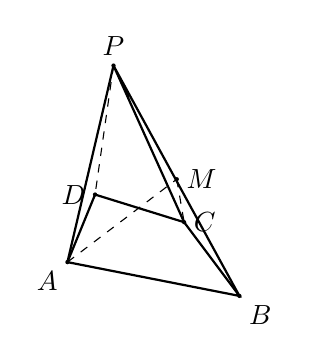
\begin{tikzpicture}[>=stealth,scale=0.78]
  \coordinate (A) at (0,0); \coordinate (B) at (2.8,-0.55);
  \coordinate (C) at (1.9,0.65); \coordinate (D) at (0.45,1.1);
  \coordinate (P) at (0.75,3.2); \coordinate (M) at (1.78,1.35);
  \draw[thick] (A)--(B)--(C)--(D)--cycle;
  \draw[thick] (P)--(A) (P)--(B) (P)--(C);
  \draw[dashed] (P)--(D) (A)--(M) (M)--(C);
  \fill (P) circle (1pt) node[above] {$P$};
  \fill (A) circle (1pt) node[below left] {$A$};
  \fill (B) circle (1pt) node[below right] {$B$};
  \fill (C) circle (1pt) node[right] {$C$};
  \fill (D) circle (1pt) node[left] {$D$};
  \fill (M) circle (1pt) node[right] {$M$};
\end{tikzpicture}
\end{center}
\nopagebreak[4]
（1） 证明：面 $PAD\perp$ 面 $PCD$；

（2） 求 $AC$ 与 $PB$ 所成的角；

（3） 求面 $AMC$ 与面 $BMC$ 所成二面角的大小。

\Needspace{4\baselineskip}
\textbf{解析}

\Needspace{5\baselineskip}
取

\nopagebreak[4]
\[
A=(0,0,0),\ B=(2,0,0),\ D=(0,1,0),\ C=(1,1,0),\ P=(0,0,1),
\]

则 $M=(1,0,1/2)$。

\gksubpart{(1)}

平面 $PAD$ 为 $x=0$，而平面 $PCD$ 内含方向向量 $(1,0,0)$，其法向量与平面 $PAD$ 的法向量垂直，因此两平面垂直。

\gksubpart{(2)}

\nopagebreak[4]
\[
\overrightarrow{AC}=(1,1,0),\qquad \overrightarrow{PB}=(2,0,-1)\text{。}
\]

\Needspace{5\baselineskip}
故

\nopagebreak[4]
\[
\cos\theta=\frac{\overrightarrow{AC}\cdot\overrightarrow{PB}}{|AC||PB|}
=\frac2{\sqrt2\sqrt5}=\sqrt{\frac25}\text{。}
\]

\gksubpart{(3)}

\Needspace{5\baselineskip}
平面 $AMC$、$BMC$ 的法向量可分别取 $(-1/2,1/2,1)$、$(-1/2,-1/2,-1)$，故锐角夹角满足

\nopagebreak[4]
\[
\cos\theta=\frac{|(-1/2,1/2,1)\cdot(-1/2,-1/2,-1)|}{(3/2)}
=\frac23\text{。}
\]

\gkanswer{答案（1）：面 $PAD\perp$ 面 $PCD$}

\gkanswer{答案（2）：$\cos\theta=\dfrac{2}{\sqrt{10}}=\sqrt{\dfrac25}$}

\gkanswer{答案（3）：两平面的锐角夹角满足 $\cos\theta=\dfrac23$}

\end{answer}
\begin{answer}
\gksolhead{19}{}

\textbf{题目}：

\Needspace{5\baselineskip}
设正项等比数列 $\{a_n\}$ 的首项 $a_1=\dfrac12$，前 $n$ 项和为 $S_n$，且

\nopagebreak[4]
\[
2^{10}S_{30}-(2^{10}+1)S_{20}+S_{10}=0\text{。}
\]

（1） 求 $\{a_n\}$ 的通项；

（2） 求 $\{nS_n\}$ 的前 $n$ 项和 $T_n$。

\Needspace{4\baselineskip}
\textbf{解析}

\gksubpart{(1)}

\Needspace{5\baselineskip}
令公比为 $q$。因 $a_1=1/2$ 且 $q>0$，把各项和写成等比和后，原条件化为

\nopagebreak[4]
\[
S_{10}q^{10}(2^{10}q^{10}-1)=0\text{。}
\]

所以 $q=1/2$，从而 $a_n=2^{-n}$，$S_n=1-2^{-n}$。于是

\gksubpart{(2)}

\nopagebreak[4]
\[
T_n=\sum_{k=1}^n kS_k
=\sum_{k=1}^n k-\sum_{k=1}^n\frac{k}{2^k}
=\frac{n(n+1)}2-2+\frac{n+2}{2^n}\text{。}
\]

\gkanswer{答案（1）：$a_n=2^{-n}$}

\gkanswer{答案（2）：$T_n=\dfrac{n(n+1)}2-2+\dfrac{n+2}{2^n}$}

\end{answer}
\begin{answer}
\gksolhead{20}{}

\textbf{题目}：

$9$ 粒种子分种在甲、乙、丙 $3$ 个坑内，每坑 $3$ 粒，每粒种子发芽的概率为 $0.5$。若一个坑内至少有 $1$ 粒种子发芽，则这个坑不需要补种；若一个坑里的种子都没发芽，则这个坑需要补种，求：

（1） 甲坑不需要补种的概率；

（2） $3$ 个坑中恰有 $1$ 个坑不需要补种的概率；

（3） 有坑需要补种的概率。（精确到 $0.001$）

\Needspace{4\baselineskip}
\textbf{解析}

\gksubpart{(1)}

\Needspace{5\baselineskip}
每个坑需要补种的概率为 $(1/2)^3=1/8$，不需要补种的概率为 $7/8$。三坑相互独立，因此

\nopagebreak[4]
\[
P(\text{\text{甲坑不需补种}})=\frac78,
\]

\gksubpart{(2)}

\nopagebreak[4]
\[
P(\text{\text{恰有一个坑不需补种}})
=\binom31\frac78\left(\frac18\right)^2
=\frac{21}{512}\approx0.041\text{，}
\]

\gksubpart{(3)}

\nopagebreak[4]
\[
P(\text{\text{有坑需补种}})=1-\left(\frac78\right)^3
=\frac{169}{512}\approx0.330\text{。}
\]

\gkanswer{答案（1）：$\dfrac78=0.875$}

\gkanswer{答案（2）：$\dfrac{21}{512}\approx0.041$}

\gkanswer{答案（3）：$\dfrac{169}{512}\approx0.330$}

\end{answer}
\begin{answer}
\gksolhead{21}{}

\textbf{题目}：

已知椭圆的中心为坐标原点 $O$，焦点在 $x$ 轴上，斜率为 $1$ 且过椭圆右焦点 $F$ 的直线交椭圆于 $A\text{、}B$ 两点，$\overrightarrow{OA}+\overrightarrow{OB}$ 与 $\vec a=(3,-1)$ 共线。

（1） 求椭圆的离心率；

（2） 设 $M$ 为椭圆上任意一点，且 $\overrightarrow{OM}=\lambda\overrightarrow{OA}+\mu\overrightarrow{OB}\ (\lambda,\mu\in\mathbb R)$，证明 $\lambda^2+\mu^2$ 为定值。

\Needspace{4\baselineskip}
\textbf{解析}

\gksubpart{(1)}

\Needspace{5\baselineskip}
设椭圆为 $x^2/a^2+y^2/b^2=1$，焦距的一半为 $c$，则 $c^2=a^2-b^2$。斜率为 $1$ 的弦所在直线为 $y=x-c$。由韦达定理，交点横坐标之和为

\nopagebreak[4]
\[
\frac{2ca^2}{a^2+b^2}\text{。}
\]

\Needspace{5\baselineskip}
向量和与 $(3,-1)$ 共线给出该横坐标和为 $3c/2$，故 $a^2=3b^2$，从而

\nopagebreak[4]
\[
e=\frac ca=\sqrt{1-\frac{b^2}{a^2}}=\frac{\sqrt6}{3}\text{。}
\]

\gksubpart{(2)}

\Needspace{5\baselineskip}
在椭圆的二次型内积 $\langle (x_1,y_1),(x_2,y_2)\rangle=x_1x_2/a^2+y_1y_2/b^2$ 下，$OA\text{、}OB$ 是单位正交向量。对任意椭圆点 $M=\lambda OA+\mu OB$，有

\nopagebreak[4]
\[
1=\langle M,M\rangle=\lambda^2+\mu^2\text{。}
\]

\gkanswer{答案（1）：$e=\dfrac{\sqrt6}{3}$}

\gkanswer{答案（2）：$\lambda^2+\mu^2=1$}

\end{answer}
\begin{answer}
\gksolhead{22}{}

\textbf{题目}：

\Needspace{5\baselineskip}
设函数

\nopagebreak[4]
\[
f(x)=x\log_2x+(1-x)\log_2(1-x)\qquad(0<x<1)\text{，}
\]

（1） 求 $f(x)$ 的最小值；

\Needspace{5\baselineskip}
（2） 设正数 $p_1,p_2,p_3,\ldots,p_{2n}$ 满足 $p_1+p_2+p_3+\cdots+p_{2n}=1$，证明

\nopagebreak[4]
\[
p_1\log_2p_1+p_2\log_2p_2+\cdots+p_{2n}\log_2p_{2n}\geqslant-n\text{。}
\]

\Needspace{4\baselineskip}
\textbf{解析}

\gksubpart{(1)}

\Needspace{5\baselineskip}
对 $f(x)$ 求导：

\nopagebreak[4]
\[
f'(x)=\log_2\frac{x}{1-x},\qquad
f''(x)=\frac1{\ln2}\left(\frac1x+\frac1{1-x}\right)>0\text{。}
\]

故唯一极小点为 $x=1/2$，最小值为 $-1$。

\gksubpart{(2)}

\Needspace{5\baselineskip}
对任意 $u,v>0$，凸函数 $t\log_2t$ 满足

\nopagebreak[4]
\[
\frac{u\log_2u+v\log_2v}{2}
\geqslant\frac{u+v}{2}\log_2\frac{u+v}{2}\text{。}
\]

\Needspace{5\baselineskip}
将 $p_1,\ldots,p_{2n}$ 两两配对并反复使用该不等式，得到

\nopagebreak[4]
\[
\sum_{i=1}^{2n}p_i\log_2p_i
\geqslant
\sum_{j=1}^{n}(p_{2j-1}+p_{2j})\log_2\frac{p_{2j-1}+p_{2j}}2
\geqslant -n\text{。}
\]

等号要求每一对相等且各对和相等，即所有 $p_i=1/(2n)$。

\gkanswer{答案（1）：最小值为 $-1$，在 $x=\dfrac12$ 时取得}

\gkanswer{答案（2）：不等式成立，且等号当且仅当 $p_1=\cdots=p_{2n}=\dfrac1{2n}$}

\end{answer}